\documentclass[acmtog]{acmart}
\usepackage{graphicx}
\usepackage{subfigure}
% Title portion
\title{Assignment 2 : Rendering mesh with texture and normal mapping} 
\author{Name:\quad xia su‘an  \\ student number:\quad 18047482
	\\email:\quad xiasa@shanghaitech.edu.cn}

% Document starts
\begin{document}
\maketitle

\vspace*{2 ex}


\section{Introduction}
\subsection{Phong lighting model and shaders}
Requirement: You are required to render a 3D object with Phong lighting model and Phong shading using OpenGL shaders and draw the model we give you in an OBJ file format.
\\Main process: Transform necessary parameters to vertex shader then to fragment shader. In fragment shader we calculate the light color ( ambient,diffuse,specular ) then output it. Also remember to set material.

\vspace*{1 ex}

\subsection{Texture and shaders}
Requirement:You are required to texture the surface of the model with OpenGL shaders.
\\Main process: Finish the function in 'my\_texture.h'. Next in fragment shader we multiple by light color.

\vspace*{1 ex}
\subsection{Normal mapping model and shaders}
Requirement:You are required to enable normal mapping for the model inside the OpenGL shaders.
\\Main process: In main.cpp, calculate the tangent and bitangent then transfor to shader to form the matrix TBN. Then in fragment shader to computer the final result.

\vspace*{2 ex}
\section{Implementation Details}
\subsection{Phong lighting model and shaders}
Detail.1: Only need to transport 'position' 'normal' 'uv' to shader in this question.
\\Detail.2: In directlight and 4 pointlight, we should calculate ambient,diffuse and specular.At last we should add them up.
\\Detail.3: The specific calculation is showed in PPT and in pointlight we should consider the attenuation.
\\Detail.4: Material is necessary. In main.cpp we can set the parametets which defined in the struct 'Material' in fragment shader.

\vspace*{1 ex}
\subsection{Texture and shaders}
Detail.1: Remeber to load and bind the picture in main.cpp.
\\Detail.2: Finish the function in 'my\_texture.h' just like what it shows in PPT.
\\Detail.3: In fragment shader, we should multiple the texturecoordinates's color by light color calculated in requirement1.

\vspace*{1 ex}
\subsection{Normal mapping model and shaders}
Detail.1: We have to additionally transport 'tangent' 'bitangent' to shader in this question.
\\Detail.2: In main.cpp, we should enlarge the original vector which hold the obj to size 14n.
\\Detail.3: Calculate each face's tangent and bitangent, which means every 3 ponit share the same  tangent and bitangent.
\\Detail.4: In vertex shader we form a 3*3 matrix TBN (Tangent,Bitangent,Normal).
\\Detail.5: In fragment shader we calculate the real final result.

\vspace*{2 ex}
\section{Results}

\begin{figure}[h]
\centering
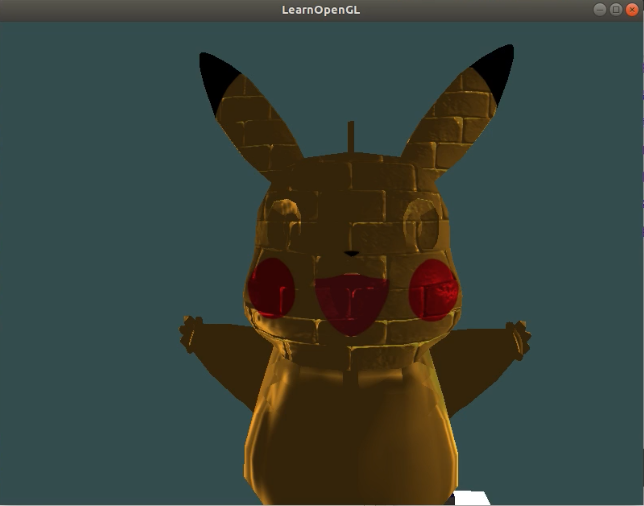
\includegraphics[width=6cm,height=6cm]{1.png}
\caption{pikaqiu\_front}
\end{figure}

\begin{figure}[h]
	\centering
	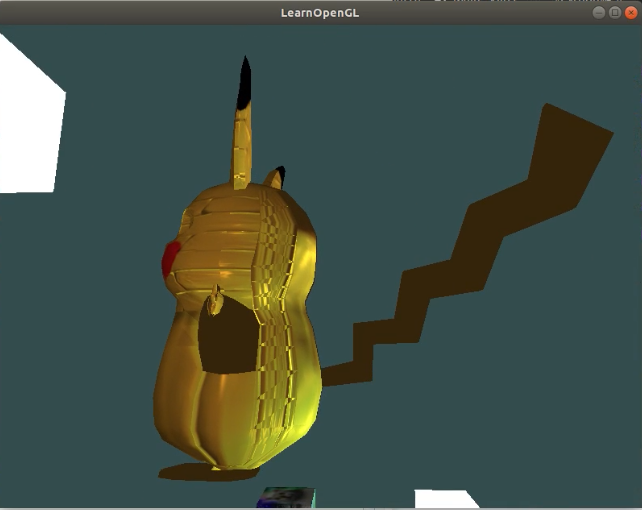
\includegraphics[width=6cm,height=6cm]{3.png}
	\caption{pikaqiu\_right}
\end{figure}

\begin{figure}[h]
	\centering
	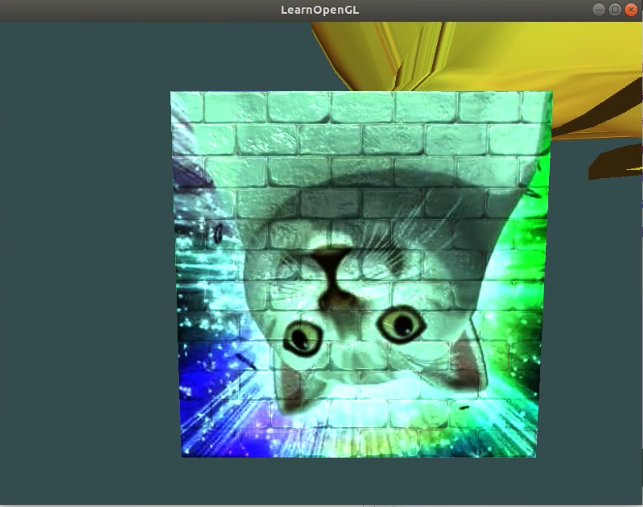
\includegraphics[width=6cm,height=6cm]{4.png}
	\caption{shocking cat}
\end{figure}
\begin{figure}[h]
	\centering
	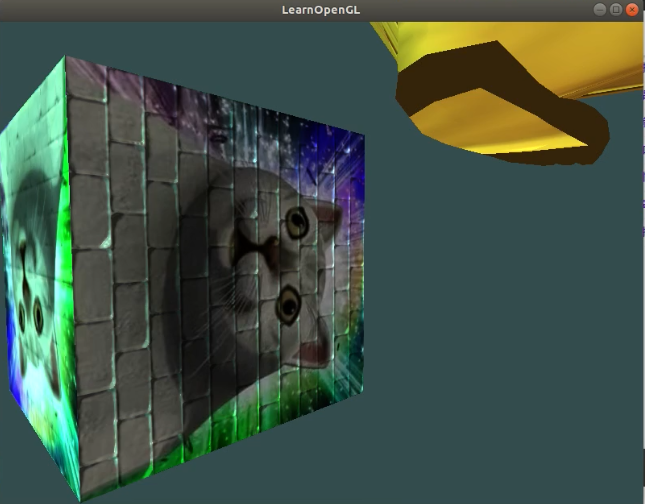
\includegraphics[width=6cm,height=6cm]{6.png}
	\caption{normal mapping1}
\end{figure}
\begin{figure}[h]
	\centering
	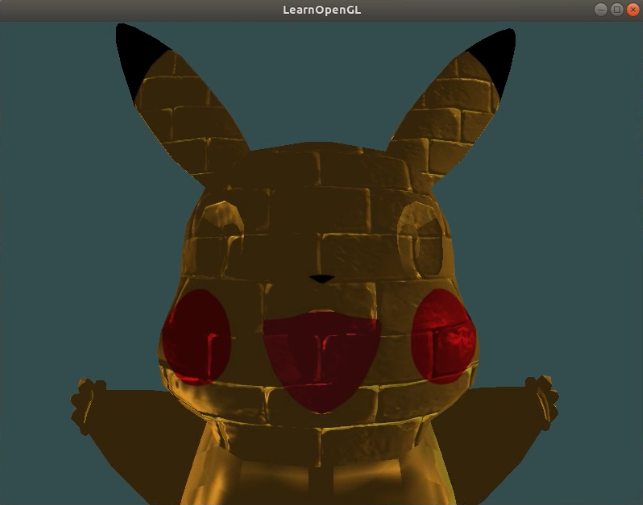
\includegraphics[width=6cm,height=6cm]{7.png}
	\caption{normal mapping2}
\end{figure}


\end{document}
